\section{Protocol}

The \textbf{blockchain} exploits the characteristics of a computer network of nodes (i.e. computers in the network with a copy of the blockchain ledger) and allows a ledger containing data and information to be managed and updated in an open, shared and distributed manner without the need for a central control and verification entity. Each blockchain is associated with a \textbf{protocol} that determines the structure of the blockchain and the way in which the blockchain handles transactions, defining its standards and modes of use.

\subsection{Zcash}

\noindent Unlike other blockchains, Zcash's blockchain allows transactions to be made, verified and recorded in two different ways: in \textbf{transparent} mode and in \textbf{shielded} mode. It is possible to distinguish the type of transaction by looking at the address prefix of the cryptocurrency involved.

\noindent Transparent addresses work like Bitcoin's, i.e. transaction data is public and visible on the blockchain. With shielded addresses, on the other hand, transactions take place without revealing the details of the transaction itself, such as the amount and addresses involved. 

\noindent In particular, there are three types of addresses, two of which are tied to their own value pool, which will henceforth be called \textbf{pool} for the sake of simplicity.

\noindent The \textbf{T} (transparent) addresses are bound to the only unshielded pool, also called the transparent pool. The transactions in this pool function like those in Bitcoin, not requiring any level of confidentiality by making each detail fully visible via a simple block explorer. As a result, it is possible to see the amount of the transaction, the starting address and the destination address.

\noindent On 28 October 2018, Zcash introduced the \textbf{Sapling} pool and \textbf{ZS} addresses, which use a ZKP (Zero-Knowledge Proof) called \textbf{zk-SNARK}. Using the Sapling pool, transaction details, such as amounts and addresses involved, are encrypted using the algorithm developed for Zcash, zk-SNARK, thus ensuring a high level of privacy and anonymity.

\noindent The Sapling pool uses a more secure and scalable version of the zk-SNARK algorithm used by the Sprout screen pool, identified with \textbf{ZC} addresses. This pool is now deprecated and no longer accessible.

\noindent On 31 May 2022, with the update called \textbf{NU5 (Network Upgrade 5)}, several new features were introduced, including \textbf{U} (unified) addresses. These types of addresses are different from addresses seen before, in that they are not linked to any particular pool, although it is a common misconception that they are linked to the \textbf{Orchard} pool, introduced with the same upgrade, NU5.

\noindent A unified address is a generic address that may contain various internal elements, known as \textbf{receivers}. This means that it can include receivers from different pools, thus allowing the customisation of one's U-address according to one's needs.

\noindent For example, we can create an address with a mix of receivers from the Transparent + Sapling + Orchard pool, Sapling + Orchard, or any other combination of pools. This offers maximum flexibility in managing one's U-address.

\noindent Another important feature of unified addresses is that they could theoretically offer the possibility of creating \textbf{multiasset} addresses, i.e. addresses that allow one to send and receive not only ZECs but also other assets, similar to Ethereum with ERC-20 tokens. This means that in the future they could be used as a platform for exchanging private digital assets, allowing parties to exchange assets without revealing transaction details.

\subsection{Verification of transactions and zk-SNARK technology}

On each blockchain, the information entered must be verified. Again, each blockchain decides how to verify this information. \textbf{Non-interactive zero-knowledge proofs} can be used in situations where there is no possibility of interaction between the demonstrator and verifier, such as in online transactions where the two parties are unable to communicate in real time. This makes non-interactive zero-knowledge proofs particularly useful in decentralised systems such as blockchains, where transactions are verified by a network of nodes and there is no central authority overseeing the verification process. Most non-interactive zero-knowledge proofs are based on mathematical constructs such as elliptic curve cryptography or coupling-based cryptography, which allow the creation of short and easily verifiable proofs of the truth of a statement. Non-interactive zero-knowledge proofs are designed to be efficient and can be used to verify a large number of statements simultaneously. To verify that transactions are correct on the blockchain, Zcash uses \textbf{zk-SNARK}, a particularly fast non-interactive zero-knowledge cryptographic proof.

\subsubsection{What is zk-SNARK}

\textbf{zk-SNARK} stands for \textbf{Zero-Knowledge Succinct Non-Interactive Argument of Knowledge} and is a type of cryptographic proof designed to guarantee the highest possible privacy. It is constructed using zero-knowledge protocols or tests (\textbf{ZKP, Zero-Knowledge Proof}), i.e. techniques that allow information to be validated and verified without having access to the information itself.

\noindent The abbreviation zk-SNARK contains the explanation of the proof itself:
\begin{itemize}
    \item \textbf{zk (Zero-Knowledge)}: a type of cryptographic proof that guarantees the confidentiality of information between users without compromising their security;
    \item \textbf{S (Succinct)}: refers to the brevity and speed with which evidence can be verified as true or legitimate. As this evidence proves the possession of information or data, its size is small, allowing it to be verified and validated in milliseconds;
    \item \textbf{N (Non-Interactive)}: indicates the absence of constant interaction between the demonstrator and the verifier. In zero-knowledge tests, it is sufficient to send a single message containing the proof to prove possession of the information, without the need for continuous or frequent communication between the parties;
    \item \textbf{ARK (Argument of Knowledge)}: refers to a proof of knowledge that the demonstrator can provide to the verifier to convince him of the possession of correct information, without revealing its content.
\end{itemize}

\noindent Basically, a zk-SNARK makes it possible to prove to a third party that you possess secret information without having to reveal it. At the same time, it provides irrefutable proof of the truthfulness of that claim. 

\subsubsection{The workings of zk-SNARK and Ali Baba's Cave of a Thousand Wonders}

The technology behind zk-SNARK is extremely complex and innovative. Its foundations were designed by cryptographers Shafi Goldwasser, Silvio Micali and Charles Rackoff in 1985. This technology makes it possible to prove knowledge of a secret without revealing it.

\noindent An explanatory example proposed by cryptographer Jean-Jacques Quisquater in 1990 may be useful to illustrate how ZKPs work.

\noindent The concept of ZKP is illustrated by means of a parabola involving the \textbf{The Cave of a Thousand Wonders of Ali Baba} (Figure \ref{fig:alibaba}).

\begin{figure}[!ht]
    \centering
    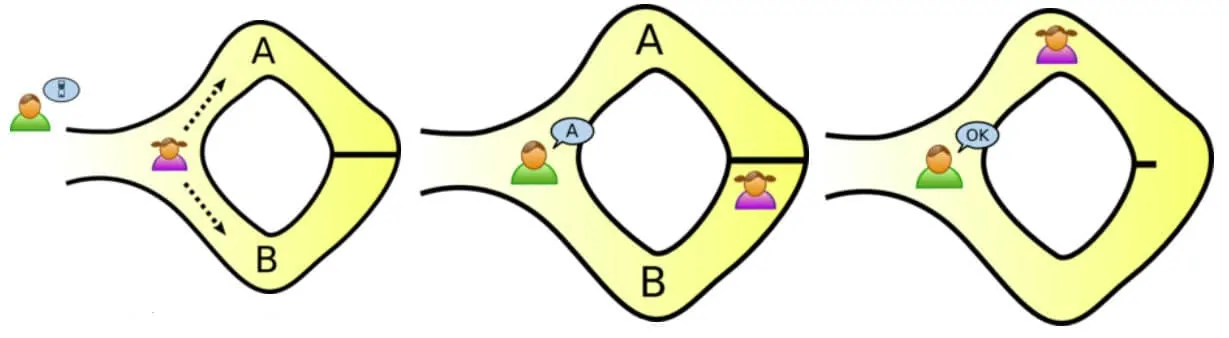
\includegraphics[width=1\linewidth]{img/alibaba.png}
    \caption{Example of Ali Baba's Cave of a Thousand Wonders}
    \label{fig:alibaba}
\end{figure}

\noindent Imagine a cave in the shape of a perfect circle, with a single entrance on the outside (the main entrance) and two paths leading to the same inner location, called the meeting point. Let these two paths be called path A and path B. Inside the cave, there is a small magic door that can only be opened by uttering the correct secret words.

\noindent Alice knows the secret words that open the magic door, while Bob wants to verify that Alice knows the secret words, but does not want Alice to reveal them to him.

\noindent How does the Zero-Knowledge Proof work?
\begin{enumerate}
    \item \textbf{Initial Position}: Alice enters the cave and chooses one of the two paths (A or B) without Bob seeing which one. She reaches the meeting point inside the cave and positions herself behind the magic door;
    \item \textbf{Bob's Choice}: Bob stands at the main entrance of the cave. From there, he calls out to Alice to come out from one of the two paths, A or B;
    \item \textbf{Alice's Response}: if Alice really knows the secret words, she can always open the magic door and exit from the path indicated by Bob. If Bob says "Path A," Alice opens the door and goes back through path A; if Bob says "Path B," Alice does the same but through path B;
    \item \textbf{Repetition of the Proof}: this process is repeated many times to reduce the probability that Alice is simply guessing the correct path. Each time, Alice randomly chooses a path (A or B) and Bob randomly asks for one of the two. After many iterations, if Alice is always able to exit from the requested path, Bob can be sure that Alice knows the secret words, as the probability that Alice correctly guesses each time becomes extremely low.
\end{enumerate}

\noindent Why is this considered a Zero-Knowledge Proof? There are essentially two reasons:
\begin{enumerate}
    \item \textbf{The secret is not revealed}: Bob never learns the secret words; he only verifies that Alice can open the magic door at any time;
    \item \textbf{Knowledge verification}: the repetition of the proof reduces the likelihood that Alice is simply guessing, convincingly demonstrating that she knows the secret words.
\end{enumerate}

\subsubsection{Importance of zk-SNARKs}

The ease with which transactions made by users can be tracked on public blockchains has led to the implementation of new security mechanisms to ensure that privacy is protected and maintained. This is essential for both users and cryptocurrencies, as privacy is a crucial element for the fungibility of digital currencies.

\noindent The implementation of privacy protocols, such as zk-SNARKs, makes it possible to guarantee the privacy of all users and participants in a blockchain network, without compromising the privacy or security of any of them. 

\noindent The use of zk-SNARKs can eliminate any kind of connection or relationship between the sender and the receiver, as well as the amounts involved in transactions. This security mechanism can be used in conjunction with other privacy technologies, such as Tor, which hides, for instance, the IP address of users. This makes privacy protection more effective in all transactions.

\subsection{Zcash and zk-SNARK}

\noindent The first cryptocurrency to apply zero-knowledge testing to ensure user privacy and security is Zcash (ZEC).

\noindent The choice to use zk-SNARK allows for a complete change in the way data is shared over the network, allowing transactions to remain encrypted while being verifiable and certifiable in terms of authenticity and validity. This offers an unprecedented level of anonymity, privacy, security and confidentiality for users.

\subsubsection{Zero Knowledge Protocol in Zcash}

The exceptional capability of the ZKP protocol to provide privacy enables the creation of an unprecedented secure communication system.

\noindent For all its properties, this privacy protocol has a wide variety of applications, ranging from military and national security implementations to secure communication and authentication systems, to cryptocurrencies and blockchain technology. In the latter field, ZKP protocols play a crucial role in protecting and maintaining the integrity of transactions conducted within the public blockchain, without revealing or leaking information among the parties involved. This is why Zcash has implemented the ZKP protocol in its system.

\subsubsection{Main features of Zcash thanks to zk-SNARK}

In Zcash, you can make transactions quickly, securely, and privately with low transaction fees of 0.0001 Zcash. Users have the option to use either fully private addresses or public and transparent addresses.

\noindent When using private addresses, information is not publicly disclosed, allowing users to include important information for the transaction recipient without exposing them to risks or vulnerabilities, as such information is protected and encrypted.

\noindent In cases where necessary, users can choose to disclose details of their transactions for auditing purposes or to comply with regulatory standards. However, the user retains full control over which transaction information they wish to reveal. Therefore, it is possible to display transferred amounts, addresses, or any related messages without revealing the identity of the sender or the recipient of the transaction.

\subsection{The elliptic curve of Zcash}

The elliptic curve of Zcash, named \textbf{Jubjub}, is a \textbf{Montgomery elliptic curve} used in cryptography for protecting sensitive data in the context of cryptocurrencies. It is designed to be efficient in both computation and cryptographic security, especially for use in zk-SNARKs.

\noindent Montgomery elliptic curves are similar to traditional elliptic curves but with a fundamental difference: the addition operation. In traditional elliptic curves, adding two points on the curve is a complex operation that requires several multiplications and inversions. In Montgomery elliptic curves, however, the addition can be performed with just one multiplication and one modular inversion. This simplification makes Montgomery elliptic curves much more efficient for cryptographic operations.

\noindent JubJub was developed by Daniel J. Bernstein and distinguishes itself from traditional elliptic curves with its notable advantages, including:

\begin{itemize}
    \item \textbf{Efficiency}: cryptographic operations performed on JubJub are faster and require less energy consumption compared to other curves;
    \item \textbf{Security}: JubJub is considered a robust elliptic curve resistant to known cryptographic attacks;
    \item \textbf{Compactness}: signatures and keys generated with JubJub are more compact than other curves, reducing transaction sizes and improving scalability.
\end{itemize}

\noindent The use of JubJub is a distinctive feature of Zcash and significantly contributes to its efficiency and privacy. The JubJub elliptic curve is employed for:

\begin{itemize}
    \item \textbf{Generating Z addresses}: Zcash addresses are anonymous and protect user privacy. JubJub is used to create these addresses securely and collision-resistant;
    \item \textbf{Encrypting transactions}: the values of Zcash transactions are encrypted to protect the confidentiality of the amounts sent. JubJub provides the mathematical basis for this encryption;
    \item \textbf{Generating anonymous signatures}: Zcash signatures allow users to spend their coins without revealing their identity. JubJub is used to create these signatures securely and anonymously.
\end{itemize}

\noindent In particular, the Montgomery curve (Figure \ref{fig:jubjub}), birationally equivalent to the JubJub curve, is defined by the equation:
\(y^2 = x^3 + 40962x^2 + x\)

\begin{figure}[!ht]
    \centering
    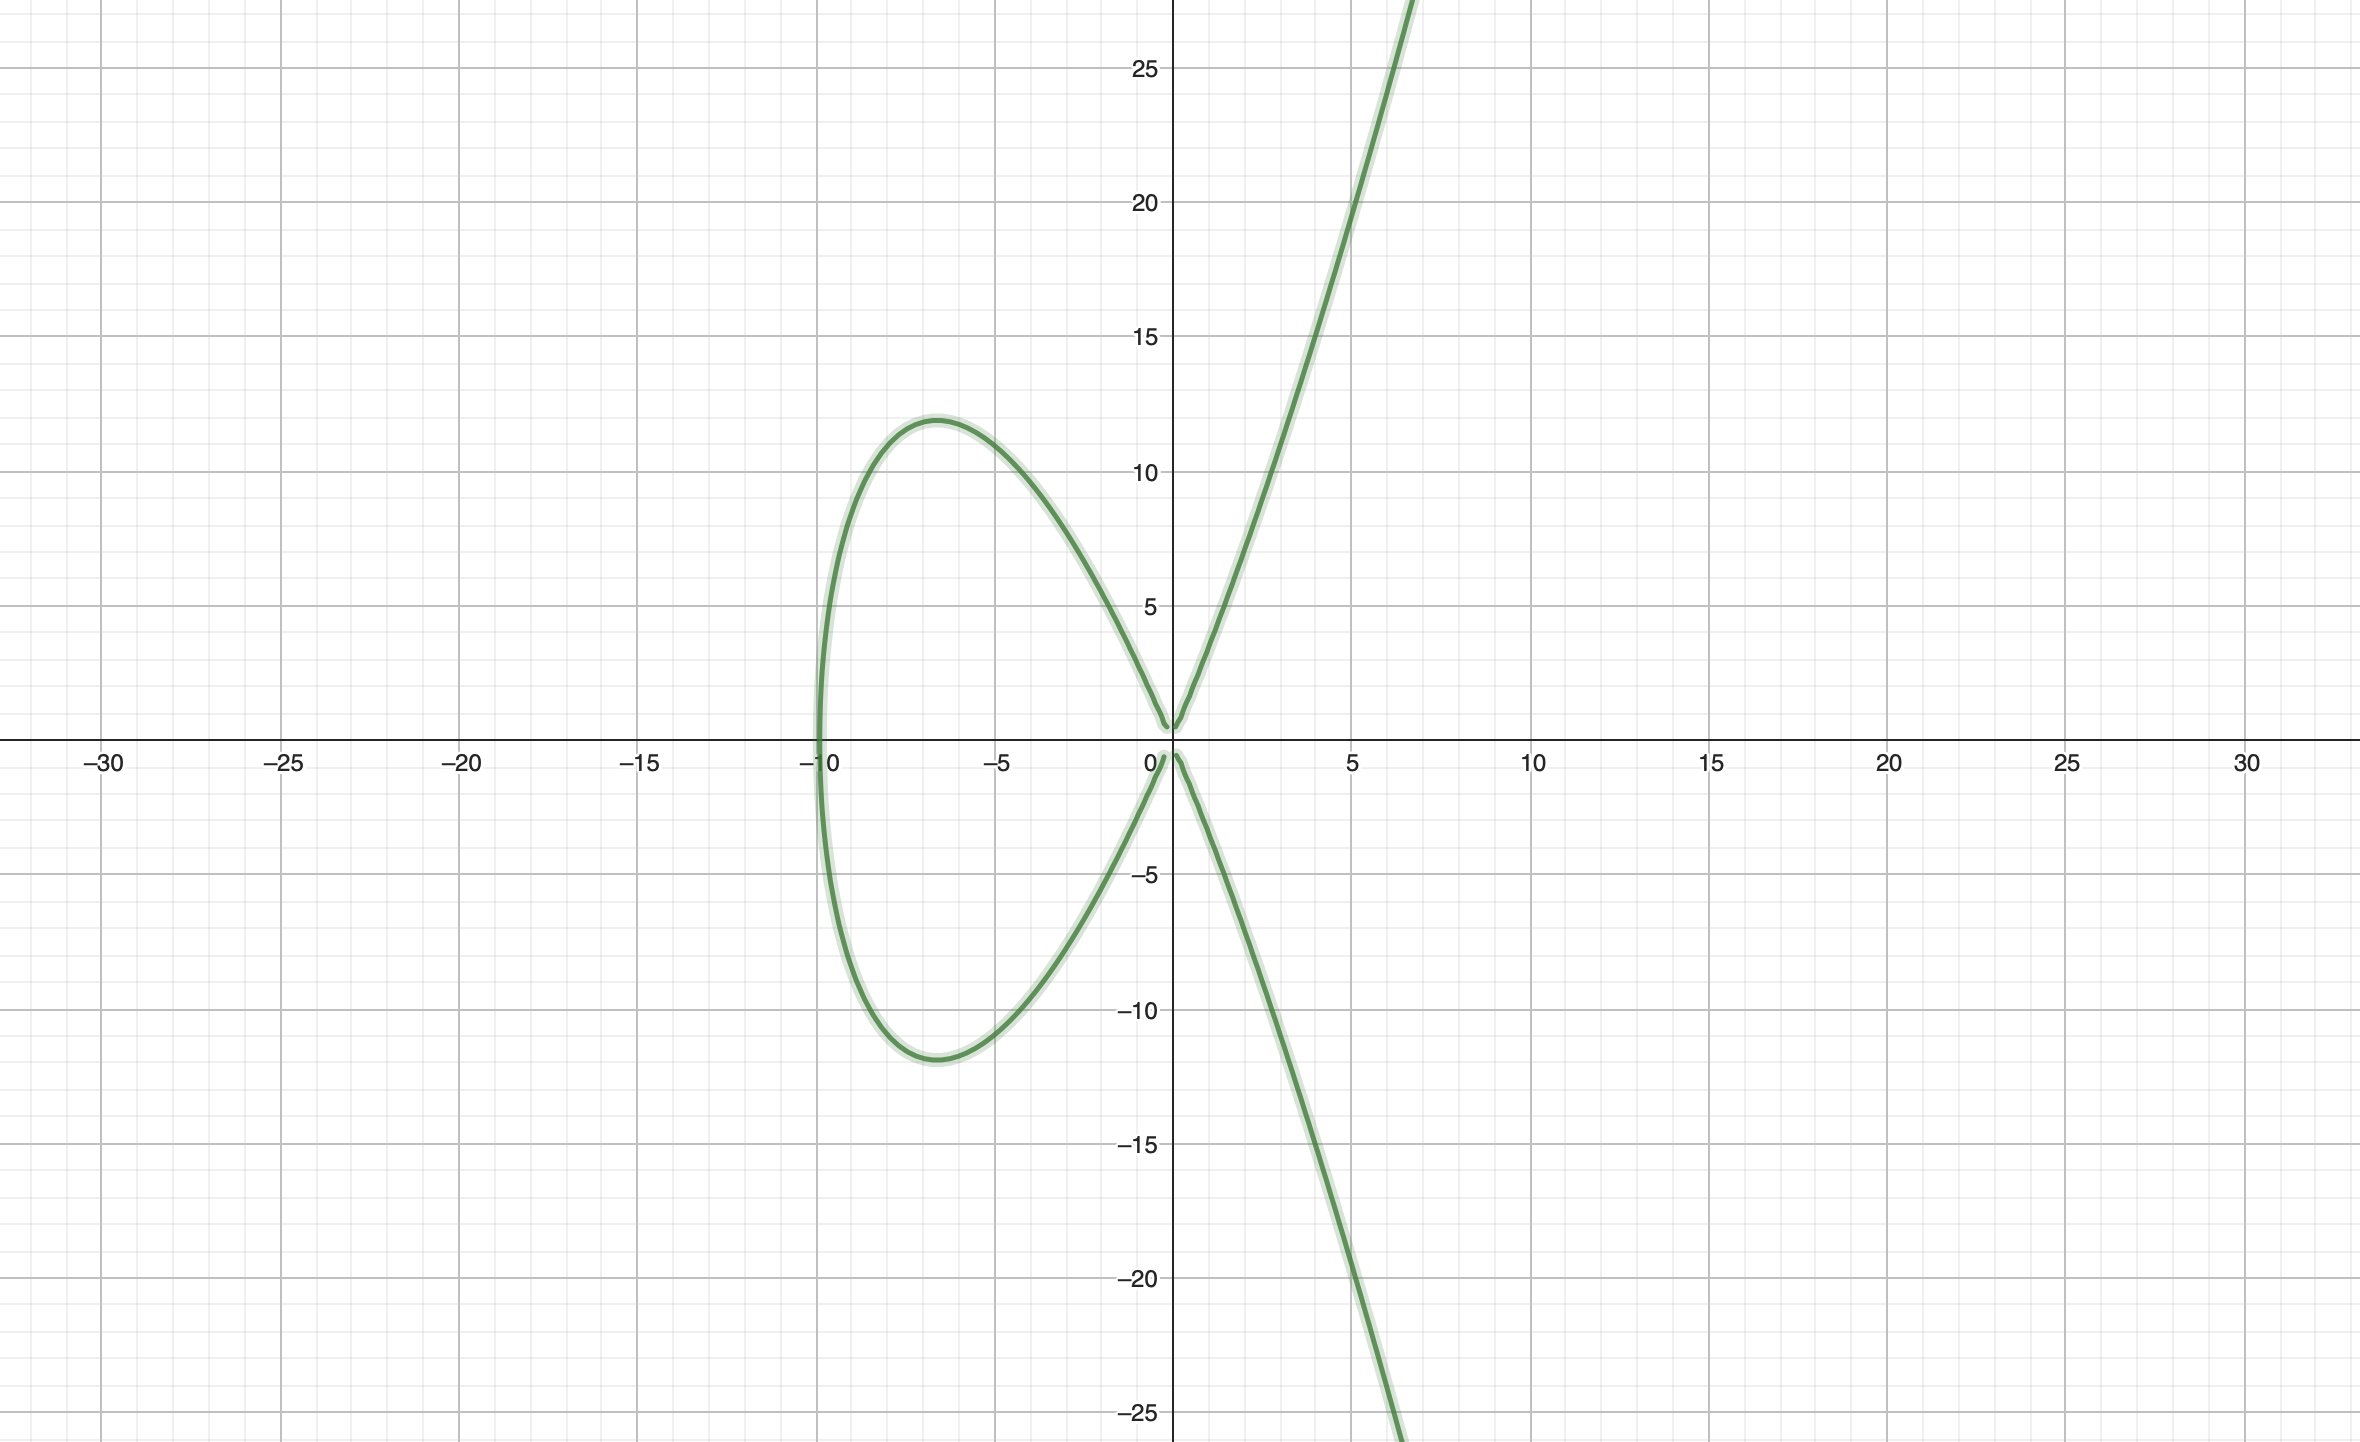
\includegraphics[width=1\linewidth]{img/jubjub.png}
    \caption{Elliptic Curve Montgomery}
    \label{fig:jubjub}
\end{figure}

\noindent Fundamentally, the JubJub elliptic curve represents a key component of Zcash technology and plays a crucial role in ensuring the privacy, security, and efficiency of transactions. Its selection represents a step forward compared to traditional elliptic curves and contributes to making Zcash one of the cryptocurrencies that most focus on user privacy.